The instances have a lot in common, but most importantly they all:
\begin{enumerate}
\item Have very large coefficients in the linear term compared to the
quadratic term.
\item All cross-product coefficients are zero in the quadratic term, i.e. in
$x^T H x$, $H$ is diagonal.
\end{enumerate}

The instances are called---based on size---\textit{small}, \textit{large}
and \textit{vlarge}.

Figure \ref{fig:histH} shows the value distribution of non-zero elements in $H$
in the three instances. Note that among all the diagonal elements of H, more
than 50 percent of them are zero, and among the non-zero elements, most of them
are less than $10^{-2}$.
\begin{figure}[ht!]
\begin{center}
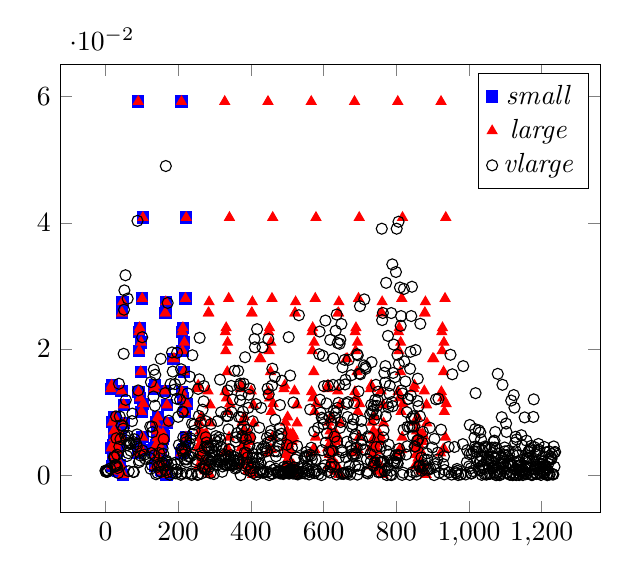
\begin{tikzpicture}
\begin{axis}[
%    xlabel={Column},
%    ylabel={Value},
    scatter/classes={
    a={mark=square*,blue},%
    b={mark=triangle*,red},%
    c={mark=o,draw=black}}]
%    b={mark=o,draw=black},
%    a={mark=o,draw=black}}]
    % \addplot[] is better than \addplot+[] here:
    % it avoids scalings of the cycle list

    \legend{\textit{small},\textit{large},\textit{vlarge}}
    \addplot[scatter,only marks,
             scatter src=explicit symbolic]
             coordinates {
(15, 0.013704) [a]
(16, 0.004299) [a]
(17, 0.014245) [a]
(18, 0.001473) [a]
(19, 0.008387) [a]
(20, 0.004771) [a]
(21, 0.003282) [a]
(22, 0.003282) [a]
(23, 0.007019) [a]
(24, 0.005940) [a]
(25, 0.009227) [a]
(26, 0.004674) [a]
(27, 0.002725) [a]
(28, 0.004941) [a]
(29, 0.005775) [a]
(30, 0.002207) [a]
(31, 0.005586) [a]
(32, 0.004039) [a]
(33, 0.006443) [a]
(34, 0.003821) [a]
(35, 0.000862) [a]
(36, 0.000643) [a]
(37, 0.005352) [a]
(38, 0.001233) [a]
(39, 0.006597) [a]
(40, 0.005749) [a]
(41, 0.001600) [a]
(42, 0.006202) [a]
(43, 0.000629) [a]
(44, 0.013353) [a]
(45, 0.025716) [a]
(46, 0.025716) [a]
(47, 0.027476) [a]
(48, 0.000099) [a]
(49, 0.000099) [a]
(50, 0.011142) [a]
(51, 0.008257) [a]
(89, 0.003500) [a]
(90, 0.059229) [a]
(91, 0.013223) [a]
(92, 0.022727) [a]
(93, 0.019726) [a]
(94, 0.023370) [a]
(95, 0.012250) [a]
(96, 0.004121) [a]
(97, 0.016391) [a]
(98, 0.021051) [a]
(99, 0.010078) [a]
(100, 0.004017) [a]
(101, 0.028020) [a]
(102, 0.006028) [a]
(103, 0.040845) [a]
(104, 0.011336) [a]
(134, 0.013704) [a]
(135, 0.004299) [a]
(136, 0.014245) [a]
(137, 0.001473) [a]
(138, 0.008387) [a]
(139, 0.004771) [a]
(140, 0.003282) [a]
(141, 0.003282) [a]
(142, 0.007019) [a]
(143, 0.005940) [a]
(144, 0.009227) [a]
(145, 0.004674) [a]
(146, 0.002725) [a]
(147, 0.004941) [a]
(148, 0.005775) [a]
(149, 0.002207) [a]
(150, 0.005586) [a]
(151, 0.004039) [a]
(152, 0.006443) [a]
(153, 0.003821) [a]
(154, 0.000862) [a]
(155, 0.000643) [a]
(156, 0.005352) [a]
(157, 0.001233) [a]
(158, 0.006597) [a]
(159, 0.005749) [a]
(160, 0.001600) [a]
(161, 0.006202) [a]
(162, 0.000629) [a]
(163, 0.013353) [a]
(164, 0.025716) [a]
(165, 0.025716) [a]
(166, 0.027476) [a]
(167, 0.000099) [a]
(168, 0.000099) [a]
(169, 0.011142) [a]
(170, 0.008257) [a]
(186, 0.018453) [a]
(189, 0.018453) [a]
(208, 0.003500) [a]
(209, 0.059229) [a]
(210, 0.013223) [a]
(211, 0.022727) [a]
(212, 0.019726) [a]
(213, 0.023370) [a]
(214, 0.012250) [a]
(215, 0.004121) [a]
(216, 0.016391) [a]
(217, 0.021051) [a]
(218, 0.010078) [a]
(219, 0.004017) [a]
(220, 0.028020) [a]
(221, 0.006028) [a]
(222, 0.040845) [a]
(223, 0.011336) [a]
(15, 0.013704) [b]
(16, 0.004299) [b]
(17, 0.014245) [b]
(18, 0.001473) [b]
(19, 0.008387) [b]
(20, 0.004771) [b]
(21, 0.003282) [b]
(22, 0.003282) [b]
(23, 0.007019) [b]
(24, 0.005940) [b]
(25, 0.009227) [b]
(26, 0.004674) [b]
(27, 0.002725) [b]
(28, 0.004941) [b]
(29, 0.005775) [b]
(30, 0.002207) [b]
(31, 0.005586) [b]
(32, 0.004039) [b]
(33, 0.006443) [b]
(34, 0.003821) [b]
(35, 0.000862) [b]
(36, 0.000643) [b]
(37, 0.005352) [b]
(38, 0.001233) [b]
(39, 0.006597) [b]
(40, 0.005749) [b]
(41, 0.001600) [b]
(42, 0.006202) [b]
(43, 0.000629) [b]
(44, 0.013353) [b]
(45, 0.025716) [b]
(46, 0.025716) [b]
(47, 0.027476) [b]
(48, 0.000099) [b]
(49, 0.000099) [b]
(50, 0.011142) [b]
(51, 0.008257) [b]
(89, 0.003500) [b]
(90, 0.059229) [b]
(91, 0.013223) [b]
(92, 0.022727) [b]
(93, 0.019726) [b]
(94, 0.023370) [b]
(95, 0.012250) [b]
(96, 0.004121) [b]
(97, 0.016391) [b]
(98, 0.021051) [b]
(99, 0.010078) [b]
(100, 0.004017) [b]
(101, 0.028020) [b]
(102, 0.006028) [b]
(103, 0.040845) [b]
(104, 0.011336) [b]
(134, 0.013704) [b]
(135, 0.004299) [b]
(136, 0.014245) [b]
(137, 0.001473) [b]
(138, 0.008387) [b]
(139, 0.004771) [b]
(140, 0.003282) [b]
(141, 0.003282) [b]
(142, 0.007019) [b]
(143, 0.005940) [b]
(144, 0.009227) [b]
(145, 0.004674) [b]
(146, 0.002725) [b]
(147, 0.004941) [b]
(148, 0.005775) [b]
(149, 0.002207) [b]
(150, 0.005586) [b]
(151, 0.004039) [b]
(152, 0.006443) [b]
(153, 0.003821) [b]
(154, 0.000862) [b]
(155, 0.000643) [b]
(156, 0.005352) [b]
(157, 0.001233) [b]
(158, 0.006597) [b]
(159, 0.005749) [b]
(160, 0.001600) [b]
(161, 0.006202) [b]
(162, 0.000629) [b]
(163, 0.013353) [b]
(164, 0.025716) [b]
(165, 0.025716) [b]
(166, 0.027476) [b]
(167, 0.000099) [b]
(168, 0.000099) [b]
(169, 0.011142) [b]
(170, 0.008257) [b]
(186, 0.018453) [b]
(189, 0.018453) [b]
(208, 0.003500) [b]
(209, 0.059229) [b]
(210, 0.013223) [b]
(211, 0.022727) [b]
(212, 0.019726) [b]
(213, 0.023370) [b]
(214, 0.012250) [b]
(215, 0.004121) [b]
(216, 0.016391) [b]
(217, 0.021051) [b]
(218, 0.010078) [b]
(219, 0.004017) [b]
(220, 0.028020) [b]
(221, 0.006028) [b]
(222, 0.040845) [b]
(223, 0.011336) [b]
(253, 0.013704) [b]
(254, 0.004299) [b]
(255, 0.014245) [b]
(256, 0.001473) [b]
(257, 0.008387) [b]
(258, 0.004771) [b]
(259, 0.003282) [b]
(260, 0.003282) [b]
(261, 0.007019) [b]
(262, 0.005940) [b]
(263, 0.009227) [b]
(264, 0.004674) [b]
(265, 0.002725) [b]
(266, 0.004941) [b]
(267, 0.005775) [b]
(268, 0.002207) [b]
(269, 0.005586) [b]
(270, 0.004039) [b]
(271, 0.006443) [b]
(272, 0.003821) [b]
(273, 0.000862) [b]
(274, 0.000643) [b]
(275, 0.005352) [b]
(276, 0.001233) [b]
(277, 0.006597) [b]
(278, 0.005749) [b]
(279, 0.001600) [b]
(280, 0.006202) [b]
(281, 0.000629) [b]
(282, 0.013353) [b]
(283, 0.025716) [b]
(284, 0.025716) [b]
(285, 0.027476) [b]
(286, 0.000099) [b]
(287, 0.000099) [b]
(288, 0.011142) [b]
(289, 0.008257) [b]
(327, 0.003500) [b]
(328, 0.059229) [b]
(329, 0.013223) [b]
(330, 0.022727) [b]
(331, 0.019726) [b]
(332, 0.023370) [b]
(333, 0.012250) [b]
(334, 0.004121) [b]
(335, 0.016391) [b]
(336, 0.021051) [b]
(337, 0.010078) [b]
(338, 0.004017) [b]
(339, 0.028020) [b]
(340, 0.006028) [b]
(341, 0.040845) [b]
(342, 0.011336) [b]
(372, 0.013704) [b]
(373, 0.004299) [b]
(374, 0.014245) [b]
(375, 0.001473) [b]
(376, 0.008387) [b]
(377, 0.004771) [b]
(378, 0.003282) [b]
(379, 0.003282) [b]
(380, 0.007019) [b]
(381, 0.005940) [b]
(382, 0.009227) [b]
(383, 0.004674) [b]
(384, 0.002725) [b]
(385, 0.004941) [b]
(386, 0.005775) [b]
(387, 0.002207) [b]
(388, 0.005586) [b]
(389, 0.004039) [b]
(390, 0.006443) [b]
(391, 0.003821) [b]
(392, 0.000862) [b]
(393, 0.000643) [b]
(394, 0.005352) [b]
(395, 0.001233) [b]
(396, 0.006597) [b]
(397, 0.005749) [b]
(398, 0.001600) [b]
(399, 0.006202) [b]
(400, 0.000629) [b]
(401, 0.013353) [b]
(402, 0.025716) [b]
(403, 0.025716) [b]
(404, 0.027476) [b]
(405, 0.000099) [b]
(406, 0.000099) [b]
(407, 0.011142) [b]
(408, 0.008257) [b]
(424, 0.018453) [b]
(427, 0.018453) [b]
(446, 0.003500) [b]
(447, 0.059229) [b]
(448, 0.013223) [b]
(449, 0.022727) [b]
(450, 0.019726) [b]
(451, 0.023370) [b]
(452, 0.012250) [b]
(453, 0.004121) [b]
(454, 0.016391) [b]
(455, 0.021051) [b]
(456, 0.010078) [b]
(457, 0.004017) [b]
(458, 0.028020) [b]
(459, 0.006028) [b]
(460, 0.040845) [b]
(461, 0.011336) [b]
(491, 0.013704) [b]
(492, 0.004299) [b]
(493, 0.014245) [b]
(494, 0.001473) [b]
(495, 0.008387) [b]
(496, 0.004771) [b]
(497, 0.003282) [b]
(498, 0.003282) [b]
(499, 0.007019) [b]
(500, 0.005940) [b]
(501, 0.009227) [b]
(502, 0.004674) [b]
(503, 0.002725) [b]
(504, 0.004941) [b]
(505, 0.005775) [b]
(506, 0.002207) [b]
(507, 0.005586) [b]
(508, 0.004039) [b]
(509, 0.006443) [b]
(510, 0.003821) [b]
(511, 0.000862) [b]
(512, 0.000643) [b]
(513, 0.005352) [b]
(514, 0.001233) [b]
(515, 0.006597) [b]
(516, 0.005749) [b]
(517, 0.001600) [b]
(518, 0.006202) [b]
(519, 0.000629) [b]
(520, 0.013353) [b]
(521, 0.025716) [b]
(522, 0.025716) [b]
(523, 0.027476) [b]
(524, 0.000099) [b]
(525, 0.000099) [b]
(526, 0.011142) [b]
(527, 0.008257) [b]
(565, 0.003500) [b]
(566, 0.059229) [b]
(567, 0.013223) [b]
(568, 0.022727) [b]
(569, 0.019726) [b]
(570, 0.023370) [b]
(571, 0.012250) [b]
(572, 0.004121) [b]
(573, 0.016391) [b]
(574, 0.021051) [b]
(575, 0.010078) [b]
(576, 0.004017) [b]
(577, 0.028020) [b]
(578, 0.006028) [b]
(579, 0.040845) [b]
(580, 0.011336) [b]
(610, 0.013704) [b]
(611, 0.004299) [b]
(612, 0.014245) [b]
(613, 0.001473) [b]
(614, 0.008387) [b]
(615, 0.004771) [b]
(616, 0.003282) [b]
(617, 0.003282) [b]
(618, 0.007019) [b]
(619, 0.005940) [b]
(620, 0.009227) [b]
(621, 0.004674) [b]
(622, 0.002725) [b]
(623, 0.004941) [b]
(624, 0.005775) [b]
(625, 0.002207) [b]
(626, 0.005586) [b]
(627, 0.004039) [b]
(628, 0.006443) [b]
(629, 0.003821) [b]
(630, 0.000862) [b]
(631, 0.000643) [b]
(632, 0.005352) [b]
(633, 0.001233) [b]
(634, 0.006597) [b]
(635, 0.005749) [b]
(636, 0.001600) [b]
(637, 0.006202) [b]
(638, 0.000629) [b]
(639, 0.013353) [b]
(640, 0.025716) [b]
(641, 0.025716) [b]
(642, 0.027476) [b]
(643, 0.000099) [b]
(644, 0.000099) [b]
(645, 0.011142) [b]
(646, 0.008257) [b]
(662, 0.018453) [b]
(665, 0.018453) [b]
(684, 0.003500) [b]
(685, 0.059229) [b]
(686, 0.013223) [b]
(687, 0.022727) [b]
(688, 0.019726) [b]
(689, 0.023370) [b]
(690, 0.012250) [b]
(691, 0.004121) [b]
(692, 0.016391) [b]
(693, 0.021051) [b]
(694, 0.010078) [b]
(695, 0.004017) [b]
(696, 0.028020) [b]
(697, 0.006028) [b]
(698, 0.040845) [b]
(699, 0.011336) [b]
(729, 0.013704) [b]
(730, 0.004299) [b]
(731, 0.014245) [b]
(732, 0.001473) [b]
(733, 0.008387) [b]
(734, 0.004771) [b]
(735, 0.003282) [b]
(736, 0.003282) [b]
(737, 0.007019) [b]
(738, 0.005940) [b]
(739, 0.009227) [b]
(740, 0.004674) [b]
(741, 0.002725) [b]
(742, 0.004941) [b]
(743, 0.005775) [b]
(744, 0.002207) [b]
(745, 0.005586) [b]
(746, 0.004039) [b]
(747, 0.006443) [b]
(748, 0.003821) [b]
(749, 0.000862) [b]
(750, 0.000643) [b]
(751, 0.005352) [b]
(752, 0.001233) [b]
(753, 0.006597) [b]
(754, 0.005749) [b]
(755, 0.001600) [b]
(756, 0.006202) [b]
(757, 0.000629) [b]
(758, 0.013353) [b]
(759, 0.025716) [b]
(760, 0.025716) [b]
(761, 0.027476) [b]
(762, 0.000099) [b]
(763, 0.000099) [b]
(764, 0.011142) [b]
(765, 0.008257) [b]
(803, 0.003500) [b]
(804, 0.059229) [b]
(805, 0.013223) [b]
(806, 0.022727) [b]
(807, 0.019726) [b]
(808, 0.023370) [b]
(809, 0.012250) [b]
(810, 0.004121) [b]
(811, 0.016391) [b]
(812, 0.021051) [b]
(813, 0.010078) [b]
(814, 0.004017) [b]
(815, 0.028020) [b]
(816, 0.006028) [b]
(817, 0.040845) [b]
(818, 0.011336) [b]
(848, 0.013704) [b]
(849, 0.004299) [b]
(850, 0.014245) [b]
(851, 0.001473) [b]
(852, 0.008387) [b]
(853, 0.004771) [b]
(854, 0.003282) [b]
(855, 0.003282) [b]
(856, 0.007019) [b]
(857, 0.005940) [b]
(858, 0.009227) [b]
(859, 0.004674) [b]
(860, 0.002725) [b]
(861, 0.004941) [b]
(862, 0.005775) [b]
(863, 0.002207) [b]
(864, 0.005586) [b]
(865, 0.004039) [b]
(866, 0.006443) [b]
(867, 0.003821) [b]
(868, 0.000862) [b]
(869, 0.000643) [b]
(870, 0.005352) [b]
(871, 0.001233) [b]
(872, 0.006597) [b]
(873, 0.005749) [b]
(874, 0.001600) [b]
(875, 0.006202) [b]
(876, 0.000629) [b]
(877, 0.013353) [b]
(878, 0.025716) [b]
(879, 0.025716) [b]
(880, 0.027476) [b]
(881, 0.000099) [b]
(882, 0.000099) [b]
(883, 0.011142) [b]
(884, 0.008257) [b]
(900, 0.018453) [b]
(903, 0.018453) [b]
(922, 0.003500) [b]
(923, 0.059229) [b]
(924, 0.013223) [b]
(925, 0.022727) [b]
(926, 0.019726) [b]
(927, 0.023370) [b]
(928, 0.012250) [b]
(929, 0.004121) [b]
(930, 0.016391) [b]
(931, 0.021051) [b]
(932, 0.010078) [b]
(933, 0.004017) [b]
(934, 0.028020) [b]
(935, 0.006028) [b]
(936, 0.040845) [b]
(937, 0.011336) [b]
(0, 0.000733) [c]
(1, 0.000562) [c]
(2, 0.000562) [c]
(3, 0.000733) [c]
(4, 0.000733) [c]
(5, 0.000562) [c]
(6, 0.000562) [c]
(7, 0.000733) [c]
(13, 0.001076) [c]
(23, 0.002873) [c]
(25, 0.002873) [c]
(26, 0.001601) [c]
(27, 0.001601) [c]
(28, 0.001456) [c]
(29, 0.009326) [c]
(30, 0.005862) [c]
(31, 0.001456) [c]
(32, 0.003255) [c]
(33, 0.001139) [c]
(35, 0.000351) [c]
(37, 0.014495) [c]
(38, 0.004533) [c]
(39, 0.009322) [c]
(41, 0.005715) [c]
(44, 0.007893) [c]
(45, 0.007893) [c]
(49, 0.007380) [c]
(50, 0.019245) [c]
(51, 0.026239) [c]
(52, 0.029297) [c]
(54, 0.006225) [c]
(55, 0.031698) [c]
(56, 0.011934) [c]
(58, 0.005524) [c]
(59, 0.003050) [c]
(60, 0.004760) [c]
(61, 0.027995) [c]
(62, 0.006278) [c]
(63, 0.003486) [c]
(64, 0.000638) [c]
(65, 0.004984) [c]
(66, 0.005233) [c]
(69, 0.003881) [c]
(70, 0.005040) [c]
(73, 0.008580) [c]
(74, 0.009763) [c]
(76, 0.000515) [c]
(78, 0.000515) [c]
(79, 0.005214) [c]
(80, 0.005693) [c]
(85, 0.004939) [c]
(86, 0.004500) [c]
(87, 0.006466) [c]
(88, 0.040320) [c]
(90, 0.013441) [c]
(92, 0.002056) [c]
(94, 0.002314) [c]
(97, 0.003098) [c]
(101, 0.021872) [c]
(102, 0.003918) [c]
(107, 0.003244) [c]
(109, 0.002625) [c]
(120, 0.002766) [c]
(123, 0.007699) [c]
(124, 0.001022) [c]
(125, 0.014762) [c]
(126, 0.003514) [c]
(127, 0.001596) [c]
(128, 0.007724) [c]
(129, 0.006812) [c]
(132, 0.012468) [c]
(133, 0.016714) [c]
(134, 0.003170) [c]
(136, 0.011017) [c]
(137, 0.015925) [c]
(139, 0.000150) [c]
(143, 0.000360) [c]
(144, 0.001338) [c]
(148, 0.003501) [c]
(149, 0.001516) [c]
(152, 0.018448) [c]
(153, 0.000539) [c]
(157, 0.004236) [c]
(158, 0.001953) [c]
(159, 0.003396) [c]
(160, 0.005719) [c]
(161, 0.001558) [c]
(164, 0.013001) [c]
(165, 0.000799) [c]
(166, 0.049011) [c]
(167, 0.002342) [c]
(168, 0.002085) [c]
(170, 0.000472) [c]
(171, 0.027306) [c]
(172, 0.001630) [c]
(174, 0.008634) [c]
(177, 0.000073) [c]
(179, 0.014448) [c]
(181, 0.001792) [c]
(182, 0.001772) [c]
(183, 0.019460) [c]
(184, 0.000429) [c]
(185, 0.016433) [c]
(189, 0.013538) [c]
(190, 0.001940) [c]
(191, 0.014448) [c]
(193, 0.000305) [c]
(194, 0.001716) [c]
(195, 0.000911) [c]
(196, 0.012132) [c]
(197, 0.019420) [c]
(198, 0.000479) [c]
(200, 0.009250) [c]
(202, 0.004789) [c]
(205, 0.011993) [c]
(206, 0.015143) [c]
(207, 0.000072) [c]
(208, 0.016797) [c]
(209, 0.004192) [c]
(210, 0.000262) [c]
(211, 0.003867) [c]
(212, 0.010100) [c]
(213, 0.009989) [c]
(214, 0.005998) [c]
(215, 0.003265) [c]
(217, 0.004192) [c]
(219, 0.002513) [c]
(220, 0.003867) [c]
(221, 0.005679) [c]
(222, 0.005242) [c]
(223, 0.000371) [c]
(224, 0.002059) [c]
(225, 0.002513) [c]
(226, 0.012971) [c]
(227, 0.004714) [c]
(229, 0.002942) [c]
(231, 0.005054) [c]
(232, 0.015625) [c]
(233, 0.002952) [c]
(234, 0.005867) [c]
(236, 0.000262) [c]
(237, 0.000049) [c]
(238, 0.008168) [c]
(239, 0.019013) [c]
(240, 0.006512) [c]
(241, 0.003254) [c]
(244, 0.008027) [c]
(245, 0.007060) [c]
(248, 0.002059) [c]
(252, 0.002416) [c]
(253, 0.000049) [c]
(255, 0.013679) [c]
(256, 0.000109) [c]
(257, 0.009387) [c]
(258, 0.015200) [c]
(259, 0.021779) [c]
(261, 0.008322) [c]
(262, 0.003437) [c]
(264, 0.000281) [c]
(265, 0.003066) [c]
(267, 0.010391) [c]
(268, 0.001267) [c]
(270, 0.011709) [c]
(271, 0.014134) [c]
(272, 0.001017) [c]
(273, 0.004300) [c]
(274, 0.000951) [c]
(275, 0.008574) [c]
(276, 0.006020) [c]
(277, 0.002431) [c]
(278, 0.005191) [c]
(279, 0.004608) [c]
(280, 0.004608) [c]
(282, 0.000891) [c]
(283, 0.004300) [c]
(284, 0.002431) [c]
(286, 0.004198) [c]
(287, 0.001370) [c]
(288, 0.002141) [c]
(289, 0.000330) [c]
(290, 0.008114) [c]
(291, 0.002010) [c]
(292, 0.004320) [c]
(293, 0.002598) [c]
(294, 0.003093) [c]
(295, 0.003187) [c]
(296, 0.002598) [c]
(297, 0.004703) [c]
(298, 0.000185) [c]
(299, 0.003762) [c]
(301, 0.005599) [c]
(304, 0.006201) [c]
(305, 0.004703) [c]
(306, 0.001623) [c]
(307, 0.002188) [c]
(308, 0.005263) [c]
(309, 0.008606) [c]
(311, 0.002481) [c]
(313, 0.006002) [c]
(314, 0.002330) [c]
(315, 0.015154) [c]
(316, 0.005599) [c]
(318, 0.009978) [c]
(319, 0.004487) [c]
(320, 0.003318) [c]
(321, 0.000545) [c]
(322, 0.001389) [c]
(326, 0.002330) [c]
(327, 0.001693) [c]
(328, 0.003280) [c]
(329, 0.001646) [c]
(330, 0.002542) [c]
(331, 0.002792) [c]
(332, 0.009392) [c]
(333, 0.001727) [c]
(335, 0.001565) [c]
(336, 0.013431) [c]
(337, 0.009392) [c]
(338, 0.007271) [c]
(339, 0.002953) [c]
(340, 0.004088) [c]
(341, 0.004088) [c]
(342, 0.001646) [c]
(343, 0.002569) [c]
(344, 0.001682) [c]
(345, 0.003179) [c]
(346, 0.014158) [c]
(347, 0.009978) [c]
(348, 0.001687) [c]
(349, 0.001553) [c]
(350, 0.011985) [c]
(352, 0.002362) [c]
(353, 0.002953) [c]
(354, 0.002291) [c]
(355, 0.016548) [c]
(356, 0.001801) [c]
(357, 0.001063) [c]
(358, 0.005356) [c]
(359, 0.006004) [c]
(360, 0.001249) [c]
(361, 0.002310) [c]
(362, 0.006686) [c]
(363, 0.001820) [c]
(365, 0.016548) [c]
(366, 0.002575) [c]
(367, 0.009246) [c]
(368, 0.001940) [c]
(369, 0.014158) [c]
(370, 0.011862) [c]
(371, 0.014518) [c]
(372, 0.000022) [c]
(373, 0.009185) [c]
(374, 0.012762) [c]
(375, 0.007216) [c]
(376, 0.006259) [c]
(377, 0.005938) [c]
(378, 0.010086) [c]
(380, 0.014518) [c]
(381, 0.007740) [c]
(383, 0.003596) [c]
(384, 0.018699) [c]
(385, 0.000919) [c]
(386, 0.005730) [c]
(387, 0.003540) [c]
(389, 0.007216) [c]
(390, 0.001687) [c]
(391, 0.002836) [c]
(392, 0.001675) [c]
(393, 0.010684) [c]
(394, 0.012762) [c]
(395, 0.004680) [c]
(396, 0.004680) [c]
(397, 0.013733) [c]
(398, 0.006004) [c]
(399, 0.000618) [c]
(400, 0.001104) [c]
(401, 0.001093) [c]
(403, 0.002735) [c]
(404, 0.002046) [c]
(405, 0.008548) [c]
(406, 0.003384) [c]
(407, 0.000335) [c]
(409, 0.001812) [c]
(410, 0.021588) [c]
(411, 0.020269) [c]
(414, 0.011266) [c]
(415, 0.000086) [c]
(416, 0.002836) [c]
(417, 0.023151) [c]
(418, 0.004301) [c]
(421, 0.001734) [c]
(422, 0.002650) [c]
(423, 0.007538) [c]
(424, 0.000466) [c]
(426, 0.000944) [c]
(427, 0.001824) [c]
(428, 0.010684) [c]
(429, 0.000773) [c]
(430, 0.004123) [c]
(431, 0.003540) [c]
(432, 0.020269) [c]
(433, 0.000374) [c]
(434, 0.000619) [c]
(435, 0.000466) [c]
(436, 0.004576) [c]
(440, 0.004260) [c]
(443, 0.003810) [c]
(444, 0.005953) [c]
(445, 0.000513) [c]
(446, 0.013733) [c]
(447, 0.005159) [c]
(448, 0.021574) [c]
(449, 0.012830) [c]
(450, 0.000019) [c]
(452, 0.001373) [c]
(453, 0.006340) [c]
(454, 0.005403) [c]
(455, 0.007017) [c]
(456, 0.000257) [c]
(458, 0.014213) [c]
(459, 0.016894) [c]
(460, 0.000237) [c]
(462, 0.000840) [c]
(465, 0.003810) [c]
(466, 0.015583) [c]
(467, 0.008779) [c]
(468, 0.001041) [c]
(469, 0.003007) [c]
(472, 0.000458) [c]
(473, 0.003776) [c]
(474, 0.000582) [c]
(475, 0.006233) [c]
(476, 0.000497) [c]
(477, 0.004755) [c]
(478, 0.000510) [c]
(479, 0.007441) [c]
(480, 0.011128) [c]
(481, 0.000268) [c]
(482, 0.000707) [c]
(483, 0.005712) [c]
(484, 0.006574) [c]
(485, 0.014978) [c]
(486, 0.000400) [c]
(488, 0.000375) [c]
(489, 0.000193) [c]
(491, 0.001323) [c]
(492, 0.000371) [c]
(494, 0.000501) [c]
(496, 0.000390) [c]
(497, 0.001040) [c]
(498, 0.001040) [c]
(499, 0.004821) [c]
(500, 0.001379) [c]
(501, 0.000591) [c]
(502, 0.000375) [c]
(503, 0.000561) [c]
(504, 0.021885) [c]
(505, 0.000243) [c]
(506, 0.000813) [c]
(507, 0.000390) [c]
(508, 0.015800) [c]
(509, 0.000927) [c]
(510, 0.000904) [c]
(511, 0.000544) [c]
(513, 0.004345) [c]
(516, 0.000257) [c]
(517, 0.011521) [c]
(518, 0.001221) [c]
(519, 0.000927) [c]
(522, 0.002484) [c]
(523, 0.000696) [c]
(524, 0.000638) [c]
(525, 0.000192) [c]
(526, 0.002825) [c]
(527, 0.004642) [c]
(528, 0.000305) [c]
(529, 0.000128) [c]
(530, 0.000561) [c]
(532, 0.025359) [c]
(540, 0.000343) [c]
(543, 0.000618) [c]
(544, 0.001106) [c]
(547, 0.002778) [c]
(548, 0.002778) [c]
(549, 0.000267) [c]
(551, 0.003046) [c]
(553, 0.003688) [c]
(555, 0.001041) [c]
(556, 0.002930) [c]
(557, 0.001679) [c]
(558, 0.000813) [c]
(560, 0.000128) [c]
(561, 0.000540) [c]
(562, 0.003267) [c]
(563, 0.010412) [c]
(566, 0.004361) [c]
(567, 0.003098) [c]
(568, 0.002499) [c]
(574, 0.006948) [c]
(575, 0.000343) [c]
(576, 0.000638) [c]
(578, 0.002499) [c]
(581, 0.000697) [c]
(585, 0.007533) [c]
(586, 0.000208) [c]
(588, 0.019178) [c]
(589, 0.022771) [c]
(590, 0.011979) [c]
(592, 0.009914) [c]
(594, 0.000022) [c]
(595, 0.009119) [c]
(596, 0.003964) [c]
(597, 0.001041) [c]
(598, 0.018930) [c]
(599, 0.008897) [c]
(600, 0.008073) [c]
(601, 0.014115) [c]
(604, 0.001576) [c]
(605, 0.024515) [c]
(606, 0.005157) [c]
(608, 0.011374) [c]
(609, 0.006632) [c]
(611, 0.000661) [c]
(612, 0.014183) [c]
(615, 0.003631) [c]
(616, 0.009245) [c]
(617, 0.000436) [c]
(618, 0.021462) [c]
(619, 0.001327) [c]
(621, 0.003826) [c]
(622, 0.001762) [c]
(623, 0.008115) [c]
(625, 0.003825) [c]
(626, 0.014316) [c]
(627, 0.018498) [c]
(628, 0.010216) [c]
(629, 0.001341) [c]
(630, 0.006099) [c]
(631, 0.009146) [c]
(633, 0.022892) [c]
(634, 0.009880) [c]
(635, 0.000115) [c]
(636, 0.025469) [c]
(637, 0.005342) [c]
(638, 0.010670) [c]
(639, 0.020960) [c]
(641, 0.011473) [c]
(642, 0.002809) [c]
(643, 0.014316) [c]
(644, 0.020833) [c]
(645, 0.007504) [c]
(646, 0.021462) [c]
(647, 0.008434) [c]
(648, 0.000242) [c]
(649, 0.023968) [c]
(650, 0.003951) [c]
(651, 0.003631) [c]
(652, 0.017116) [c]
(653, 0.000313) [c]
(654, 0.000201) [c]
(655, 0.000305) [c]
(656, 0.000305) [c]
(657, 0.000314) [c]
(658, 0.018285) [c]
(659, 0.014385) [c]
(660, 0.015126) [c]
(661, 0.002846) [c]
(662, 0.000415) [c]
(663, 0.011303) [c]
(664, 0.005304) [c]
(665, 0.000246) [c]
(666, 0.009229) [c]
(667, 0.011584) [c]
(668, 0.000563) [c]
(669, 0.018285) [c]
(671, 0.001470) [c]
(673, 0.000099) [c]
(674, 0.004584) [c]
(676, 0.015846) [c]
(677, 0.003873) [c]
(678, 0.007658) [c]
(679, 0.003363) [c]
(680, 0.008077) [c]
(681, 0.003112) [c]
(682, 0.008849) [c]
(683, 0.005812) [c]
(684, 0.011425) [c]
(685, 0.003447) [c]
(687, 0.001435) [c]
(688, 0.006430) [c]
(689, 0.003363) [c]
(691, 0.004357) [c]
(692, 0.019178) [c]
(693, 0.000096) [c]
(694, 0.019014) [c]
(695, 0.001514) [c]
(696, 0.013279) [c]
(698, 0.016125) [c]
(699, 0.000939) [c]
(700, 0.026796) [c]
(701, 0.016001) [c]
(703, 0.004849) [c]
(704, 0.008611) [c]
(705, 0.007271) [c]
(706, 0.005506) [c]
(709, 0.004088) [c]
(711, 0.017411) [c]
(712, 0.027870) [c]
(714, 0.004026) [c]
(715, 0.017138) [c]
(716, 0.016880) [c]
(718, 0.000377) [c]
(719, 0.002549) [c]
(721, 0.000642) [c]
(722, 0.000270) [c]
(723, 0.006146) [c]
(727, 0.005965) [c]
(728, 0.009697) [c]
(729, 0.003355) [c]
(730, 0.002220) [c]
(731, 0.011143) [c]
(732, 0.017920) [c]
(733, 0.010060) [c]
(736, 0.010275) [c]
(737, 0.001480) [c]
(738, 0.010999) [c]
(739, 0.008849) [c]
(740, 0.002009) [c]
(742, 0.011959) [c]
(744, 0.014328) [c]
(745, 0.004490) [c]
(746, 0.009631) [c]
(747, 0.010999) [c]
(748, 0.002386) [c]
(749, 0.011894) [c]
(750, 0.013240) [c]
(751, 0.000476) [c]
(752, 0.000480) [c]
(755, 0.002063) [c]
(756, 0.000498) [c]
(757, 0.004560) [c]
(758, 0.002063) [c]
(759, 0.002063) [c]
(760, 0.039076) [c]
(761, 0.024591) [c]
(762, 0.002063) [c]
(763, 0.025722) [c]
(764, 0.006001) [c]
(765, 0.007126) [c]
(766, 0.002141) [c]
(767, 0.016243) [c]
(768, 0.000662) [c]
(769, 0.014662) [c]
(770, 0.017300) [c]
(771, 0.009322) [c]
(772, 0.030494) [c]
(773, 0.003842) [c]
(774, 0.000022) [c]
(775, 0.011305) [c]
(776, 0.001189) [c]
(777, 0.022090) [c]
(778, 0.010763) [c]
(779, 0.004848) [c]
(780, 0.003276) [c]
(781, 0.012926) [c]
(782, 0.014212) [c]
(784, 0.000077) [c]
(785, 0.000709) [c]
(786, 0.025704) [c]
(787, 0.000022) [c]
(788, 0.011596) [c]
(789, 0.033423) [c]
(790, 0.010939) [c]
(791, 0.016216) [c]
(792, 0.002255) [c]
(793, 0.020711) [c]
(794, 0.001845) [c]
(795, 0.002059) [c]
(796, 0.015542) [c]
(798, 0.003145) [c]
(799, 0.032213) [c]
(800, 0.002688) [c]
(801, 0.039076) [c]
(802, 0.002017) [c]
(803, 0.019086) [c]
(804, 0.001841) [c]
(805, 0.003229) [c]
(806, 0.040177) [c]
(807, 0.017609) [c]
(808, 0.004201) [c]
(809, 0.003089) [c]
(810, 0.029750) [c]
(812, 0.023679) [c]
(813, 0.025229) [c]
(814, 0.013441) [c]
(816, 0.000050) [c]
(817, 0.012946) [c]
(819, 0.000404) [c]
(820, 0.007205) [c]
(821, 0.029531) [c]
(822, 0.018035) [c]
(825, 0.014857) [c]
(827, 0.003273) [c]
(829, 0.009990) [c]
(830, 0.004585) [c]
(831, 0.007677) [c]
(832, 0.012078) [c]
(833, 0.012098) [c]
(836, 0.007655) [c]
(837, 0.000050) [c]
(838, 0.016873) [c]
(839, 0.019562) [c]
(840, 0.012634) [c]
(841, 0.025229) [c]
(842, 0.009004) [c]
(843, 0.029874) [c]
(844, 0.007705) [c]
(845, 0.000495) [c]
(846, 0.006250) [c]
(847, 0.009342) [c]
(849, 0.007705) [c]
(850, 0.004550) [c]
(851, 0.009004) [c]
(852, 0.004550) [c]
(853, 0.019842) [c]
(855, 0.000591) [c]
(856, 0.000103) [c]
(857, 0.005470) [c]
(858, 0.011772) [c]
(859, 0.015309) [c]
(860, 0.005615) [c]
(861, 0.010956) [c]
(863, 0.001539) [c]
(864, 0.001378) [c]
(865, 0.009342) [c]
(866, 0.024001) [c]
(869, 0.002808) [c]
(870, 0.000683) [c]
(872, 0.005150) [c]
(873, 0.006877) [c]
(874, 0.001420) [c]
(875, 0.001612) [c]
(876, 0.001033) [c]
(878, 0.002452) [c]
(884, 0.003455) [c]
(885, 0.000868) [c]
(886, 0.002451) [c]
(888, 0.001027) [c]
(892, 0.007525) [c]
(894, 0.000981) [c]
(899, 0.004402) [c]
(904, 0.000026) [c]
(905, 0.005756) [c]
(907, 0.001769) [c]
(908, 0.001335) [c]
(909, 0.012037) [c]
(913, 0.002508) [c]
(914, 0.003579) [c]
(916, 0.012132) [c]
(918, 0.000387) [c]
(923, 0.007225) [c]
(929, 0.001762) [c]
(931, 0.002965) [c]
(932, 0.000135) [c]
(933, 0.000821) [c]
(944, 0.004485) [c]
(945, 0.000457) [c]
(949, 0.019093) [c]
(952, 0.000101) [c]
(954, 0.015999) [c]
(960, 0.004485) [c]
(963, 0.000481) [c]
(965, 0.000287) [c]
(967, 0.000991) [c]
(968, 0.000698) [c]
(970, 0.000026) [c]
(977, 0.000153) [c]
(978, 0.000147) [c]
(983, 0.004926) [c]
(984, 0.017295) [c]
(991, 0.000124) [c]
(994, 0.002040) [c]
(995, 0.003961) [c]
(1000, 0.001396) [c]
(1001, 0.003342) [c]
(1002, 0.007964) [c]
(1005, 0.001107) [c]
(1006, 0.000245) [c]
(1007, 0.000350) [c]
(1008, 0.003451) [c]
(1011, 0.000653) [c]
(1013, 0.003753) [c]
(1015, 0.005970) [c]
(1016, 0.004527) [c]
(1017, 0.007311) [c]
(1018, 0.013008) [c]
(1019, 0.004194) [c]
(1020, 0.003741) [c]
(1021, 0.002764) [c]
(1025, 0.004362) [c]
(1026, 0.001016) [c]
(1027, 0.007122) [c]
(1028, 0.004315) [c]
(1029, 0.000737) [c]
(1030, 0.002246) [c]
(1031, 0.006787) [c]
(1032, 0.002149) [c]
(1033, 0.005676) [c]
(1034, 0.003041) [c]
(1035, 0.000063) [c]
(1036, 0.003994) [c]
(1037, 0.001641) [c]
(1038, 0.001172) [c]
(1040, 0.001641) [c]
(1042, 0.001214) [c]
(1043, 0.000166) [c]
(1044, 0.004554) [c]
(1046, 0.004271) [c]
(1047, 0.004439) [c]
(1048, 0.000092) [c]
(1049, 0.002329) [c]
(1050, 0.003015) [c]
(1051, 0.000212) [c]
(1052, 0.001712) [c]
(1053, 0.002516) [c]
(1054, 0.002246) [c]
(1055, 0.002235) [c]
(1056, 0.001104) [c]
(1057, 0.000203) [c]
(1058, 0.004188) [c]
(1059, 0.000377) [c]
(1060, 0.002337) [c]
(1061, 0.002270) [c]
(1062, 0.002267) [c]
(1063, 0.004376) [c]
(1064, 0.003509) [c]
(1065, 0.001098) [c]
(1066, 0.002970) [c]
(1067, 0.005290) [c]
(1068, 0.001363) [c]
(1069, 0.000384) [c]
(1070, 0.005484) [c]
(1071, 0.004386) [c]
(1072, 0.006852) [c]
(1073, 0.002641) [c]
(1074, 0.000026) [c]
(1075, 0.000026) [c]
(1076, 0.004288) [c]
(1077, 0.000377) [c]
(1078, 0.000875) [c]
(1079, 0.016067) [c]
(1080, 0.003372) [c]
(1082, 0.000617) [c]
(1084, 0.000026) [c]
(1085, 0.000026) [c]
(1086, 0.000285) [c]
(1087, 0.001767) [c]
(1088, 0.002020) [c]
(1089, 0.002793) [c]
(1090, 0.009200) [c]
(1091, 0.000800) [c]
(1092, 0.014330) [c]
(1093, 0.001730) [c]
(1094, 0.002676) [c]
(1095, 0.001730) [c]
(1096, 0.003221) [c]
(1097, 0.002168) [c]
(1098, 0.004398) [c]
(1099, 0.003786) [c]
(1100, 0.001504) [c]
(1101, 0.003101) [c]
(1102, 0.008191) [c]
(1103, 0.006863) [c]
(1104, 0.000431) [c]
(1105, 0.000321) [c]
(1107, 0.001910) [c]
(1108, 0.003867) [c]
(1109, 0.001465) [c]
(1110, 0.003320) [c]
(1111, 0.002078) [c]
(1112, 0.000075) [c]
(1113, 0.000094) [c]
(1115, 0.001633) [c]
(1116, 0.011836) [c]
(1117, 0.000441) [c]
(1119, 0.001534) [c]
(1120, 0.000014) [c]
(1121, 0.003298) [c]
(1123, 0.012705) [c]
(1124, 0.000143) [c]
(1125, 0.010712) [c]
(1126, 0.000932) [c]
(1127, 0.005152) [c]
(1128, 0.006086) [c]
(1129, 0.003795) [c]
(1130, 0.000022) [c]
(1131, 0.005672) [c]
(1132, 0.000932) [c]
(1133, 0.003127) [c]
(1134, 0.002181) [c]
(1135, 0.002052) [c]
(1136, 0.001500) [c]
(1137, 0.000766) [c]
(1138, 0.000028) [c]
(1139, 0.000282) [c]
(1140, 0.000766) [c]
(1141, 0.000834) [c]
(1142, 0.001539) [c]
(1143, 0.001223) [c]
(1144, 0.006338) [c]
(1145, 0.000591) [c]
(1146, 0.004734) [c]
(1147, 0.000462) [c]
(1148, 0.000027) [c]
(1149, 0.000819) [c]
(1150, 0.000312) [c]
(1151, 0.002550) [c]
(1152, 0.000333) [c]
(1153, 0.009163) [c]
(1154, 0.000395) [c]
(1155, 0.002457) [c]
(1156, 0.000163) [c]
(1157, 0.001376) [c]
(1158, 0.005478) [c]
(1159, 0.000212) [c]
(1160, 0.001942) [c]
(1161, 0.002752) [c]
(1162, 0.003028) [c]
(1163, 0.003681) [c]
(1164, 0.003786) [c]
(1165, 0.002682) [c]
(1166, 0.002705) [c]
(1168, 0.003951) [c]
(1169, 0.004189) [c]
(1170, 0.000112) [c]
(1171, 0.004654) [c]
(1173, 0.000014) [c]
(1174, 0.002238) [c]
(1176, 0.000112) [c]
(1177, 0.009243) [c]
(1178, 0.012024) [c]
(1179, 0.004472) [c]
(1180, 0.001086) [c]
(1181, 0.000893) [c]
(1182, 0.001407) [c]
(1183, 0.003307) [c]
(1184, 0.001385) [c]
(1185, 0.000186) [c]
(1186, 0.000336) [c]
(1187, 0.002116) [c]
(1188, 0.003887) [c]
(1189, 0.000937) [c]
(1190, 0.001366) [c]
(1191, 0.004956) [c]
(1192, 0.004056) [c]
(1193, 0.001005) [c]
(1194, 0.003708) [c]
(1195, 0.000249) [c]
(1196, 0.001811) [c]
(1197, 0.001157) [c]
(1198, 0.000046) [c]
(1200, 0.001796) [c]
(1201, 0.001731) [c]
(1202, 0.000576) [c]
(1203, 0.002872) [c]
(1204, 0.001776) [c]
(1205, 0.000309) [c]
(1206, 0.000884) [c]
(1207, 0.004478) [c]
(1208, 0.000346) [c]
(1209, 0.001218) [c]
(1210, 0.001544) [c]
(1211, 0.000728) [c]
(1212, 0.003636) [c]
(1213, 0.001129) [c]
(1214, 0.000192) [c]
(1215, 0.000011) [c]
(1216, 0.000122) [c]
(1218, 0.001798) [c]
(1219, 0.002491) [c]
(1220, 0.000122) [c]
(1221, 0.003760) [c]
(1222, 0.000122) [c]
(1225, 0.002876) [c]
(1226, 0.002522) [c]
(1227, 0.002679) [c]
(1228, 0.003357) [c]
(1229, 0.000124) [c]
(1230, 0.000199) [c]
(1232, 0.000122) [c]
(1233, 0.004560) [c]
(1234, 0.003556) [c]
(1235, 0.001338) [c]
(1237, 0.003692) [c]
};
\end{axis}
\end{tikzpicture}

\end{center}
\caption{Value distribution of non-zero elements in $H$. The y-axis represent
the value of each element, while the x-axis represent which column index the
element is located.}
\label{fig:histH}
\end{figure}
Note that no non-zero elements in the linear term in any of the instances
has absolute value less than 20. We see that the values in the linear term
are generally of much higher magnitude than the values in the quadratic term.

\begin{table}[ht!]
    \centering
    \caption{Problem size of each instance}
    \begin{tabular}{lrrr}
    Problem size & \textit{small} & \textit{large} & \textit{vlarge} \\\hline
    Rows         & 82             & 328            & 1127 \\
    Columns      & 238            & 952            & 3437 \\
    Non-zeroes A & 348            & 1392           & 4840 \\
    Non-zeroes H & 108            & 432            & 894 \\
    \end{tabular}
    \label{table:sizes}
\end{table}

Let us take a look at some hard statistics of each instance.
Table \ref{table:sizes} shows the problem size of each instance.
Table \ref{table:maxmin} shows some statistics about the non-zero elements in
the objective function for $i = 1,2,\ldots,n$ where $n$ is the number of
columns.
\begin{table}[ht!]
    \centering
    \caption{Statistics on the Non-zero values in the objective function of
each instance.}

    \begin{tabular}{lrr}
      & \textit{small} and \textit{large}         & \textit{vlarge} \\\hline
    $\max(h_{ii})$      & $2.9614 \times 10^{-2}$ & $4.9011 \times 10^{-2}$ \\
    $\min(h_{ii})$      & $4.9290 \times 10^{-5}$ & $1.1026 \times 10^{-5}$ \\
$\textrm{mean}(h_{ii})$ & $5.2864 \times 10^{-3}$ & $5.8984 \times 10^{-3}$ \\
    $\max(b_{i})$       & 20                      & 20 \\
    $\min(b_{i})$       & -70                     & -50 \\
    \end{tabular}
    \label{table:maxmin}
\end{table}
The rows and columns in each problem represent vertices and edges respectively.
An avid reader might notice that \textit{small} and \textit{large} are very
much alike.
That is entirely justified as \textit{large} is four \textit{small}-networks
connected forming one large network.

For each of these instances, Goodtech wants to solve several versions
with slight variations in the input.
If one or more variables in an instance is forced to zero, it forms a new
instance that we refer to as a $\emph{subinstance}$ of the original instance.
Goodtech wants to simulate that all combinations of edges in the network
fail, by forcing their corresponding variables to zero.
This means that for each of the three instances described in this chapter,
they ideally want to solve a total of $2^n - 1$ subinstances. While this is
unrealistic, it is unlikely that all edges in the network breaks down.
A more realistic approach is to try to solve all subinstances with no more than
$b$ breakdowns. That is, for some given $b$ and a problem size $n$, we solve
$s(b, n) = \sum_{j=0}^b {\binom{n}{j}}$ subinstances with less than or equal to
$b$ breakdowns.
